\chapter{Defining some concepts and redefining the variables} 
\section{Voices, parts and strata}\label{section:parts-and-strata}
Before we start this section, we need to look at some vocabulary to make sure we understand what we are discussing. The most important definition (and distinction) we will introduce is the definition of the terms \textit{part} and \textit{stratum}. The need for these definitions arises from the increasing complexity of the rules of counterpoint when it is generalised to three voices. Indeed, the rules are no longer (as we shall see later) concerned solely with the counterpoints and the \cf, but also with new concepts, such as that referred to by Fux as 'the lowest voice'. As the term 'voice' is too generic (it is used in Fux's text to describe notions as different as 'counterpoint', '\cf', voice range and the so called 'lowest voice'), we need to create a precise vocabulary that is different from the word 'voice' to talk about these new concepts. 


With this in mind, let's explain what 'parts' and 'strata' are, and how they relate to the concept of 'voice'.

\subsubsection{Voices} Again, voices are that vague and \textit{general} concept, whereas parts and strata are more precise and \textit{specific} concepts. The concept of 'voice' includes both 'parts' and 'strata'. In other words, each of these two concepts is a type of voice. When we talk about a voice, we could be talking about either a part or a stratum. To make a metaphor out of it, we could say that parts and strata are a type of voice.

Since there are as many parts and layers as there are voices, in a composition with $n$ voices there will also be $n$ parts and $n$ layers.

\subsubsection{Parts}
Parts are an intuitive and concrete concept because each part corresponds to what a particular person sings or what a particular instrument plays. They correspond to a staff (each staff corresponds to a part). The term 'part' is the same as that used by Fux in his \gap. The three parts in a three-part composition are: the \cf, the first \cps and the second \cp. Fux distinguishes them by calling them by the name of their range, i.e. "bass", "tenor", "alto" or "soprano" (obviously you cannot have all four in a three-part composition).

\subsubsection{Strata}
As for the strata, they are defined like this: a stratum delineates discrete layers or levels of pitches at any given moment in the composition. It denotes a vertical alignment of simultaneous notes and organizes them into distinct strata. By definition, the lowest stratum encompasses the lowest sounding notes, the highest stratum comprises the highest sounding notes, and intermediary strata represent pitch levels in between.
This concept is very helpful in identifying and categorising the vertical placement of pitches, creating distinct categories of sound within the overall texture of the counterpoint composition. It provides a way of analysing and understanding the distribution of pitches across different parts, allowing more complex rules to be established: for example, it would now be possible to establish a rule between the notes of the cantus firmus and the highest sounding notes (no matter which part they come from). The full potential of strata lies in harmonic rules, but as we shall see, some melodic rules are also related to it.

\begin{minipage}{0.6\textwidth}
    The term stratum was chosen in this context for its visual impact. In geology, a stratum "is a rock layer with a lithology (texture, colour, grain size, composition, fossils, etc.) different from the adjacent ones", see figure \ref{fig:geological-strata}.
    \end{minipage}
    \hfill
    \begin{minipage}{0.3\textwidth}
      \centering
      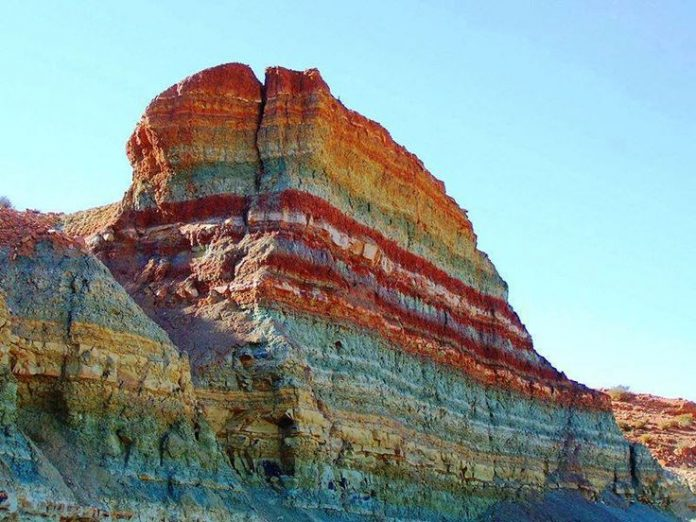
\includegraphics[width=\textwidth]{Images/rainbow-sediment.jpg}
      \captionof{figure}{Geological strata, for the illustration}
      \label{fig:geological-strata}
\end{minipage}
\vspace{.5cm}

When Fux speaks about the lowest stratum, he often uses the word 'bass'. It was deliberately chosen to speak about the 'lowest stratum' instead of the 'bass' (like Fux does), because 'bass' is also the name of a range of voices (on a par with soprano and alto, for example), and there is already enough complexity in all the terminology to add even further ambiguity. 

\paragraph{}
These new terms (parts and strata) are used where the distinction between the concepts is important. Whenever this distinction is not relevant, the more general term 'voice' is used to reduce the complexity of reading. In this case, the 'voice' could refer to both a stratum and a part.

Since a picture is worth a thousand words, Figure \ref{fig:lowest} illustrates the difference between parts (the blue lines) and strata (the red and orange lines). The lowest stratum is shown in its own colour (red) because it is the most meaningful stratum, and it will be particularly important later on.

\begin{figure}[h]
  \centering
  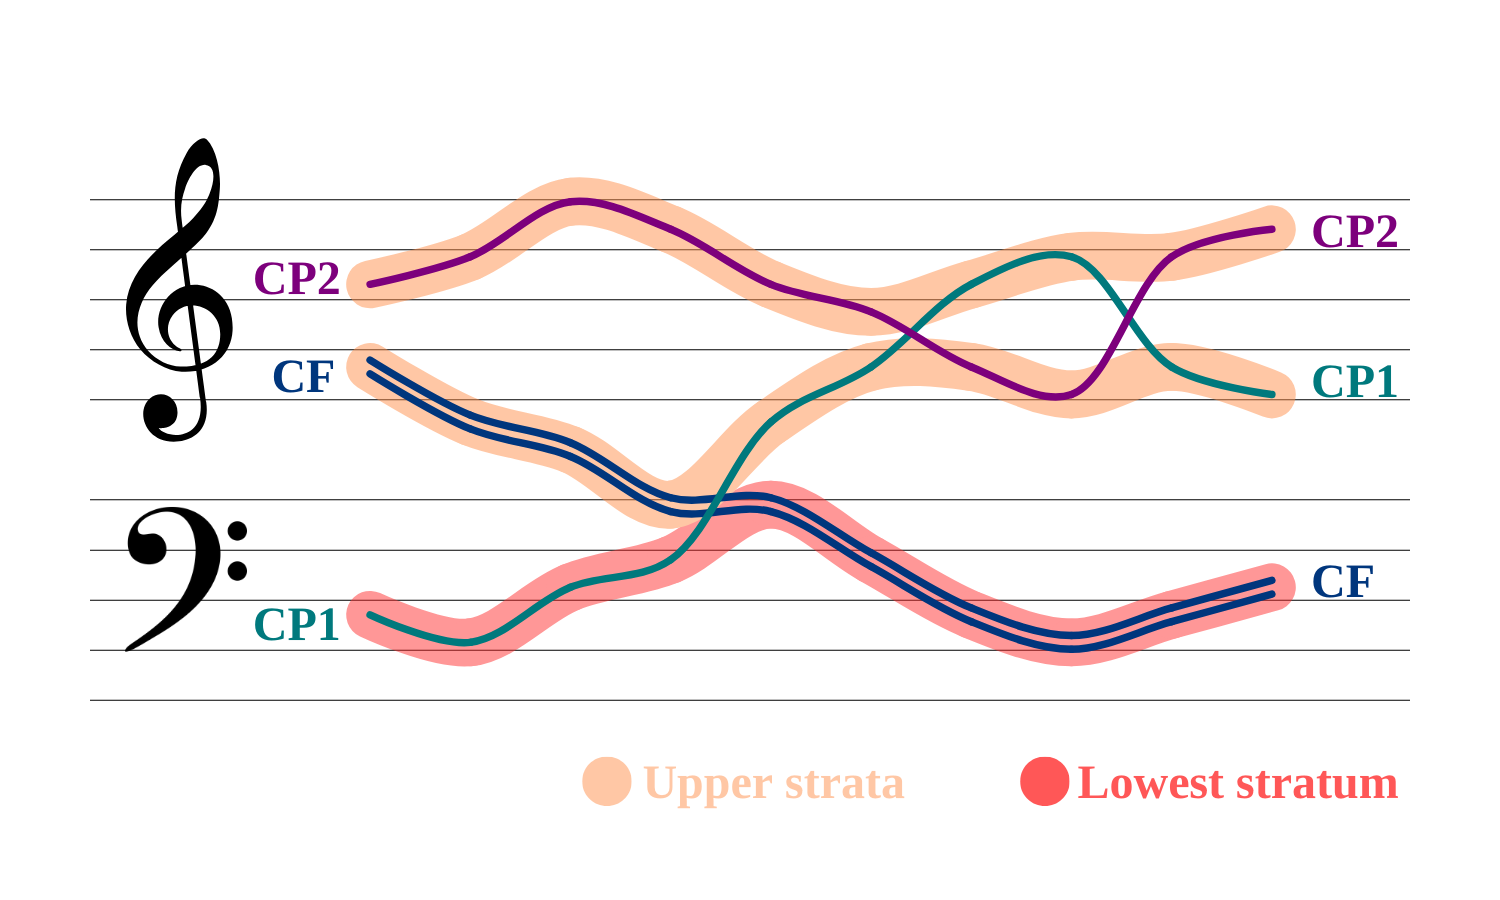
\includegraphics[width=1\textwidth]{Images/strata_example.png}
  \caption{Parts and strata in a three voice composition}
  \label{fig:lowest}
\end{figure}


Here is also the mathematical representation for the notes of the lowest stratum (written $N(a)$, see section \ref{section:changes induced} for the notations):
% todo a, b, c, et A
\begin{equation}
    \forall i \in [0, 3] \quad \forall j \in [0, m-1): N(a)[i,j] = \text{min} (N(cf)[i,j], N(cp_1)[i,j], N(cp_2)[i,j])
\end{equation}

Of the first upper stratum, or medium stratum (written $N(b)$, see section \ref{section:changes induced} for the notations):
\begin{equation}
    \forall i \in [0, 3] \quad \forall j \in [0, m-1): N(b)[i,j] = \text{med}\footnote{Where $\text{med}(X)$ means the median value of X.} (N(cf)[i,j], N(cp_1)[i,j], N(cp_2)[i,j])
\end{equation}

And of the second upper stratum, or uppest stratum (written $N(c)$, see section \ref{section:changes induced} for the notations):
\begin{equation}
    \forall i \in [0, 3] \quad \forall j \in [0, m-1): N(c)[i,j] = \text{max} (N(cf)[i,j], N(cp_1)[i,j], N(cp_2)[i,j])
\end{equation}

\subsubsection{One part per stratum and one stratum per part} \label{subsubsection:one-part-per-stratum}
It is important to note that, for each musical measure, there is a bijection between the individual parts and the corresponding strata. This means that, for any given measure, each stratum uniquely corresponds to a single part, and vice versa. Put differently, if two parts within a measure share the same pitch, they do not constitute the same stratum. Instead, one part corresponds with one stratum, and the other one to a separate stratum.

To illustrate this, consider a scenario in a two-voice composition (see figure \ref{fig:one-voice-max-can-be-a}), where part 'cf' and part 'cp1' in measure X both have a pitch value of 67 (representing a G). Despite having identical pitches at the same moment, one part is categorised as the lowest stratum, while the other is designated as the uppermost stratum. This distinction becomes crucial for subsequent analysis, especially when calculating aspects like motions.

To know which part gets to be the lowest stratum in such situations, an arbitrary hierarchical rule is implemented. If the ambivalence is between the \cfs and another part, the \cfs is always prioritised and assigned the role of the lowest stratum, over any other part. In the case of a ambivalence between the first \cp and the second \cp, the first \cps is given the status of the lowest stratum. 

\begin{figure}[h]
    \centering
    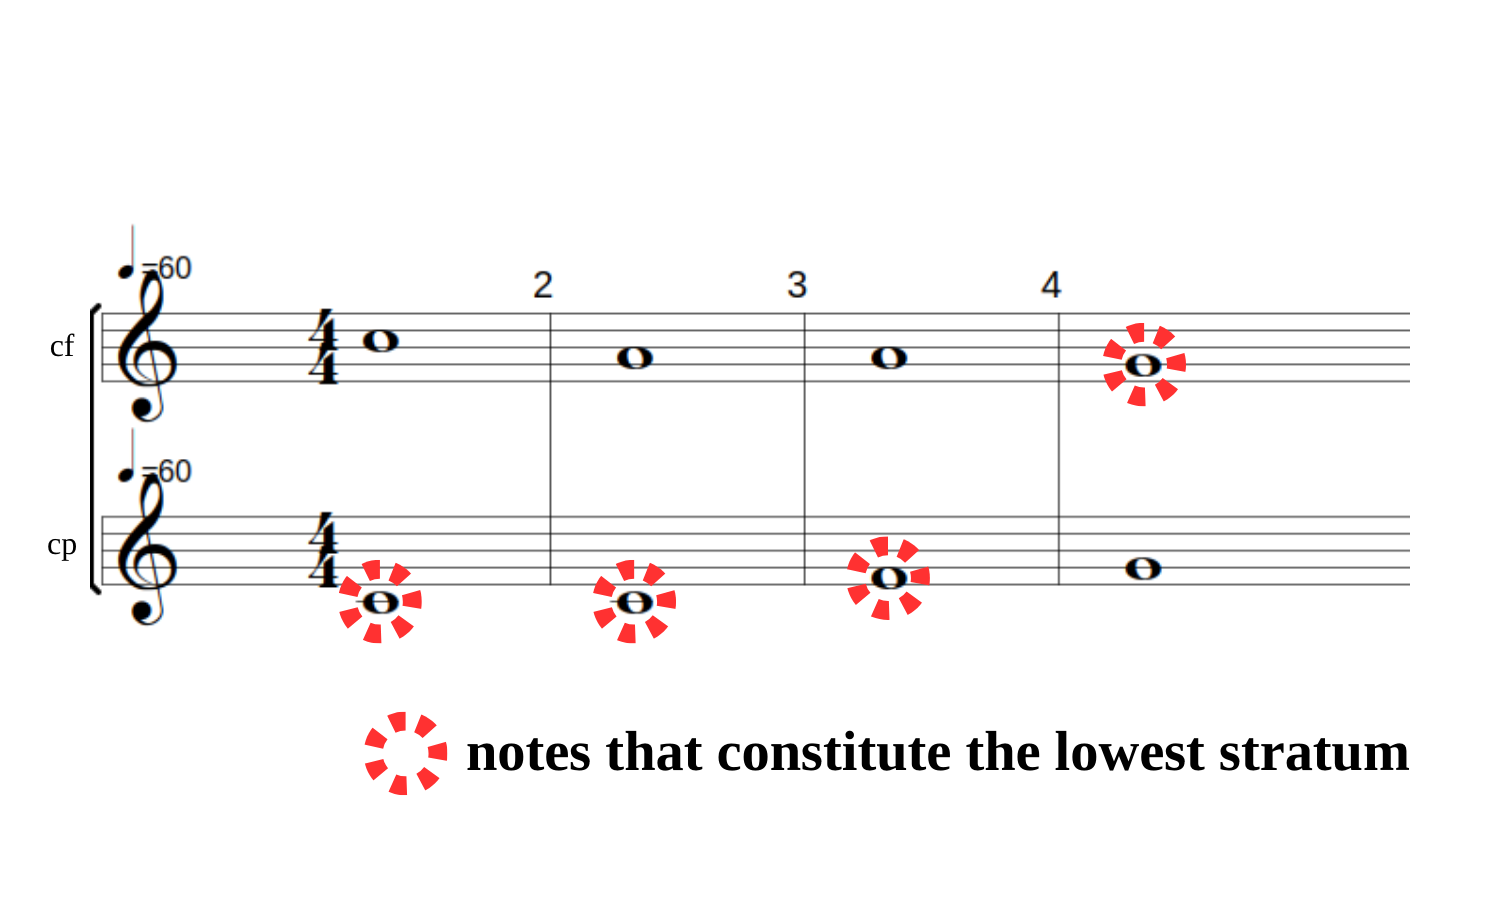
\includegraphics[width=.5\textwidth]{Images/one-voice-max-can-be-a.png}
    \caption{Establishing which part corresponds to the lowest stratum}
    \label{fig:one-voice-max-can-be-a}
  \end{figure}

\section{Exploring the interaction of the parts with the lowest stratum} \label{exploring-interaction-p-a}

One of the major differences between the composition of two voices (i.e., one \cfs and one counterpoint) and the generalisation to three voices (i.e., one \cfs and two counterpoints) is that the rules no longer necessarily apply between the counterpoints and the \cf, but instead of this are mostly applied \textbf{between the different parts and the lowest stratum}. 

If we go back to the rules for two voices, we see that each of them applied between the single counterpoint and the \cf. For example, when it was stated that each interval must be consonant, this referred to the interval between the counterpoint and the \cf.
On the other hand, in his second part (where he describes the rules for composing in three voices), Fux explains that the rules are not necessarily to be observed between each of the counterpoints and the \cf, but rather between "each of the voices and the lowest voice" (i.e. the lowest stratum). Again, if we take the example of the need for consonance between the voices, consonance will be required in the intervals between the notes of any voice and those of the lowest voice (whether or not the latter is the \cf).
Fux approaches the concept of lowest stratum without ever stating it clearly, mentioning for example that the lowest voice can change (sometimes the bass is the lowest voice, sometimes the tenor, ...), and that at any given moment the lowest voice should be considered. In other words, Fux says that the rules apply between the parts and the lowest stratum.

\subsubsection{Generalisation of two-voice counterpoint}
One might be tempted to conclude that three-part composition breaks completely with two-part composition, but that would be too hasty a conclusion. Indeed, on closer inspection, the way the rules worked in two-part composition (from counterpoint to \textit{cantus firmus}) is just one particular case of this new vision of things. In two-part composition, too, the rules apply between the parts and the lowest stratum. But of course, since there were only two voices, the lowest stratum was either counterpoint or cantus firmus. This means that when links were established between the upper part and the lowest stratum, links were also established between the counterpoint and the cantus firmus. Considering the rules as being established between the counterpoint and the \cfs was just a simplification of reality, although it was perfectly correct. We were therefore considering a convenient particular case, and not the general case. Please note that when we talk about "applying constraints from voice A to voice B", it is clear that the constraints are bidirectional and that they also apply from voice B to voice A. What is shown here is rather the philosophy behind the application of these constraints, and the reasons why they were imposed.

The particular case happening when composing with two parts is illustrated in figures \ref{fig:cp2cf-2v} and \ref{fig:p2l-2v}. As we can see on those pseudo-compositions, it does not change anything to apply the constraints between the counterpoints and the \cfs or between the parts and the lowest stratum.

\vspace{.5cm}
\begin{minipage}{0.46\textwidth}
    \centering
    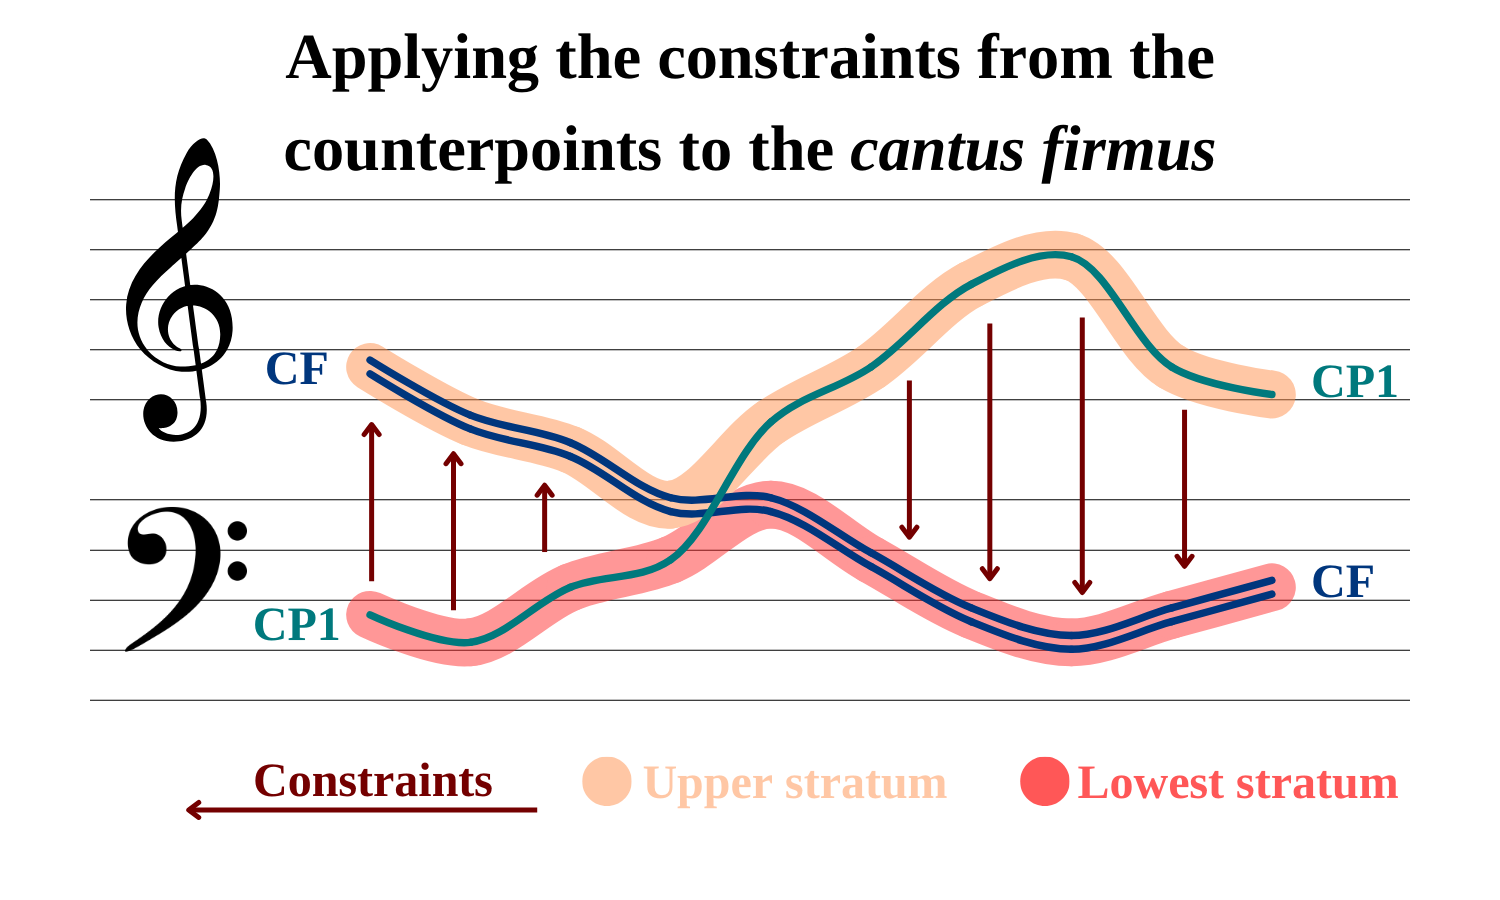
\includegraphics[width=\textwidth]{Images/cp2cf-2v.png}
    \captionof{figure}{Applying the constraints from the \cps to the \cf}
    \label{fig:cp2cf-2v}
    \end{minipage}
    \hfill
    \begin{minipage}{0.46\textwidth}
      \centering
      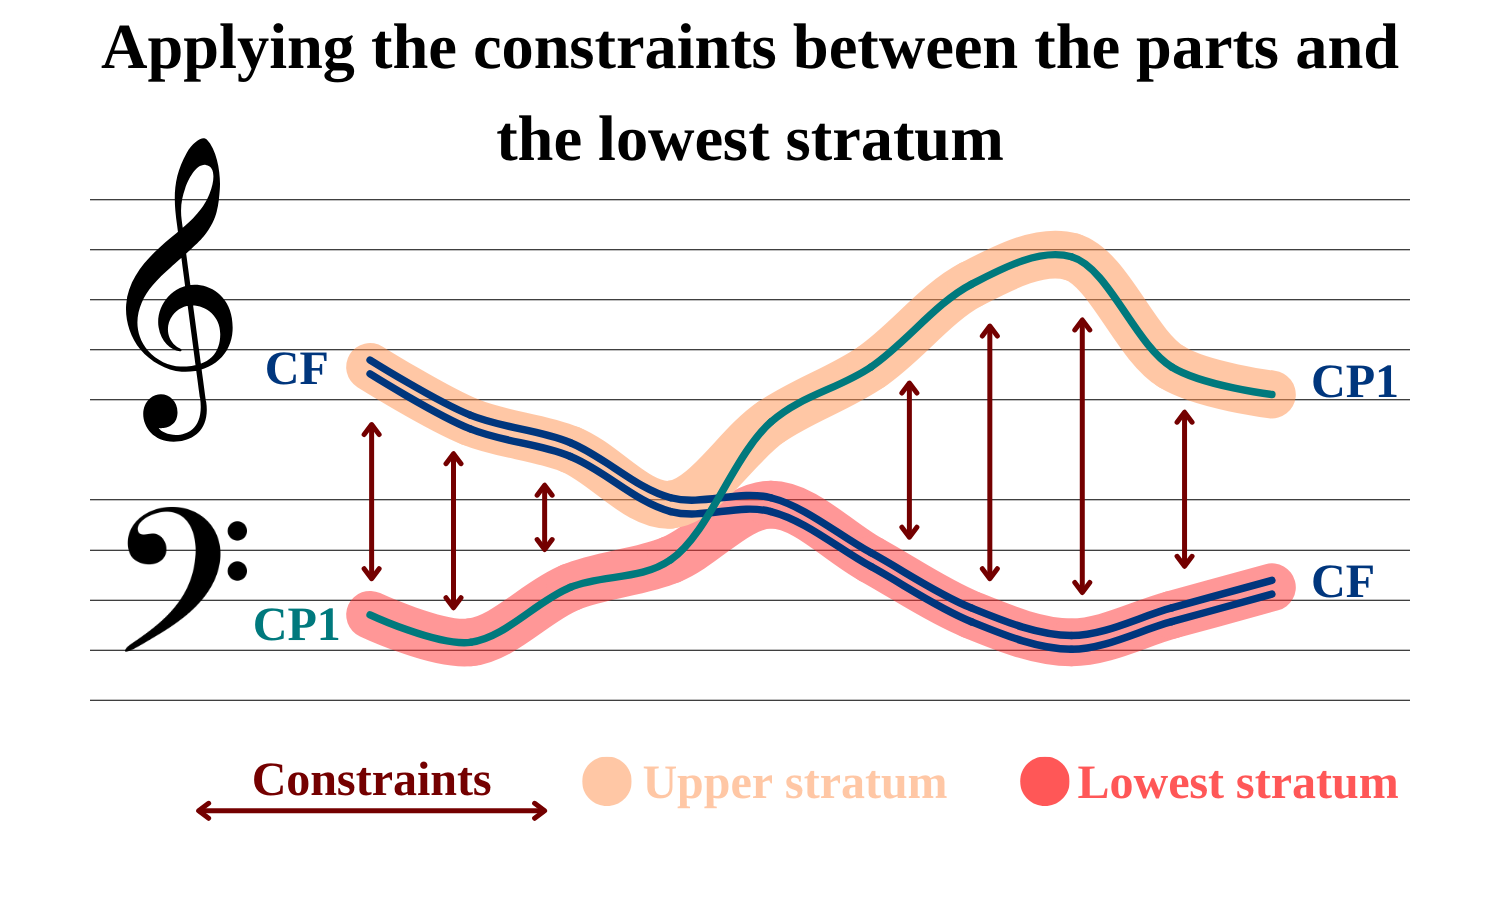
\includegraphics[width=\textwidth]{Images/p2l-2v.png}
      \captionof{figure}{Applying the constraints from the parts to the lowest stratum}
      \label{fig:p2l-2v}
\end{minipage}
\vspace{.5cm}

However, when it comes to generalising the composition of counterpoint for three voices, the same simplification is no longer possible. We are now forced to establish our rules between the parts and the lowest stratum, and no longer between the counterpoints and the \cf. In figures \ref{fig:cp2cf-3v} and \ref{fig:p2l-3v} it becomes clear that establishing the rules between the counterpoints and the \cfs is really different from applying them between the various parts to the lowest stratum. In these figures, the parts don't intersect and therefore fit perfectly with the strata, so the constraints are always applied to the same counterpoint. This was done for the sake of intelligibility of the graphs, but it is of course possible for the parts to cross and for the "target" of the constraints not always to be the same counterpoint.

\vspace{.5cm}
\begin{minipage}{0.46\textwidth}
    \centering
    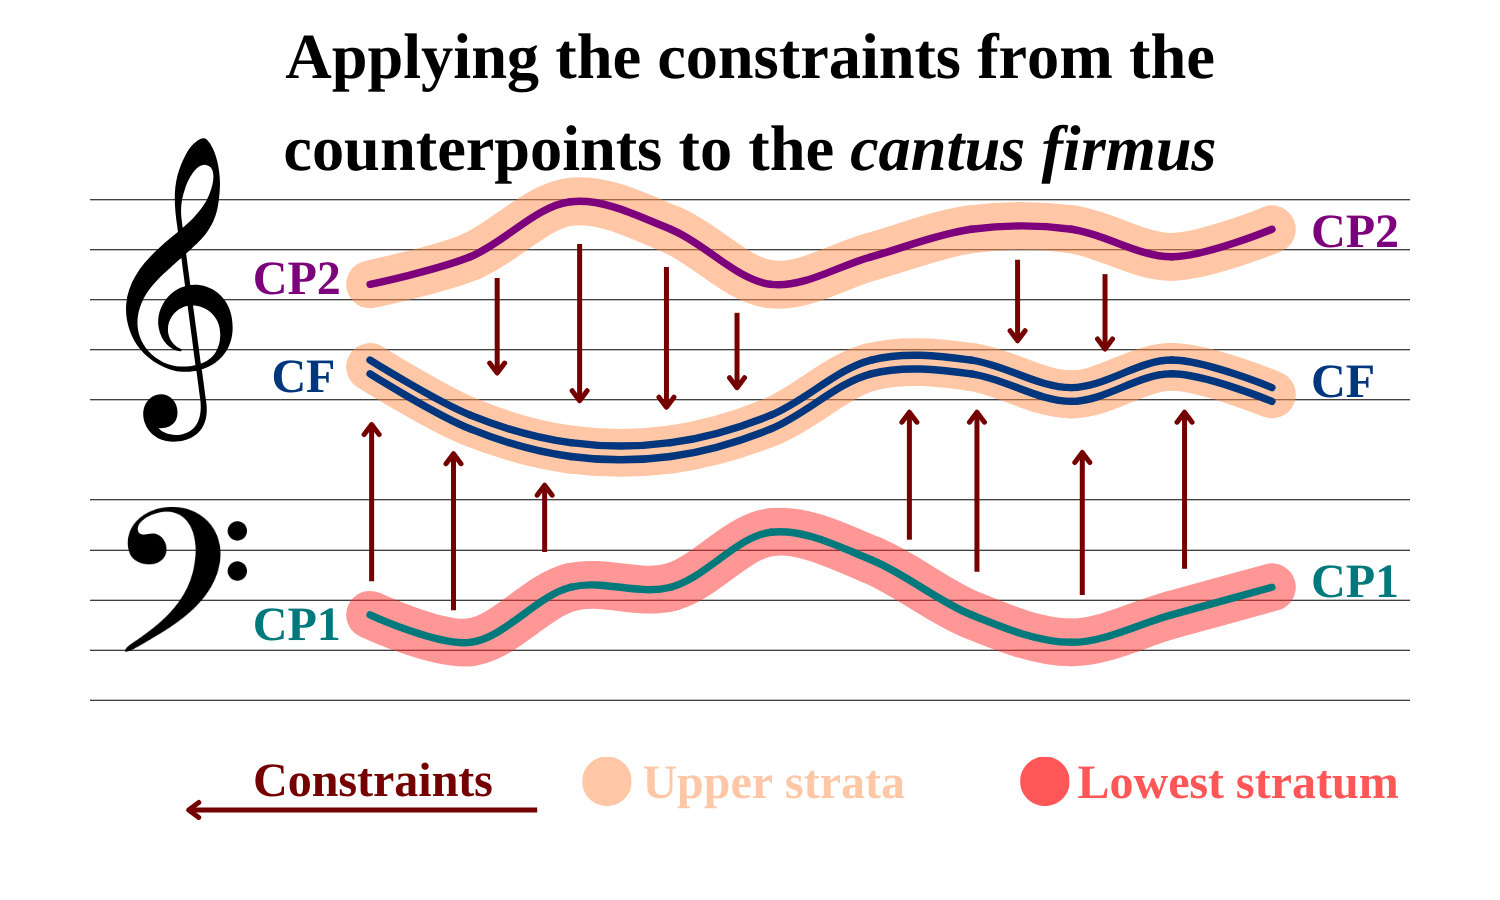
\includegraphics[width=\textwidth]{Images/cp2cf-3v.png}
    \captionof{figure}{Wrong approach: applying the constraints between the \cps to the \cf.}
    \label{fig:cp2cf-3v}
    \end{minipage}
    \hfill
    \begin{minipage}{0.46\textwidth}
      \centering
      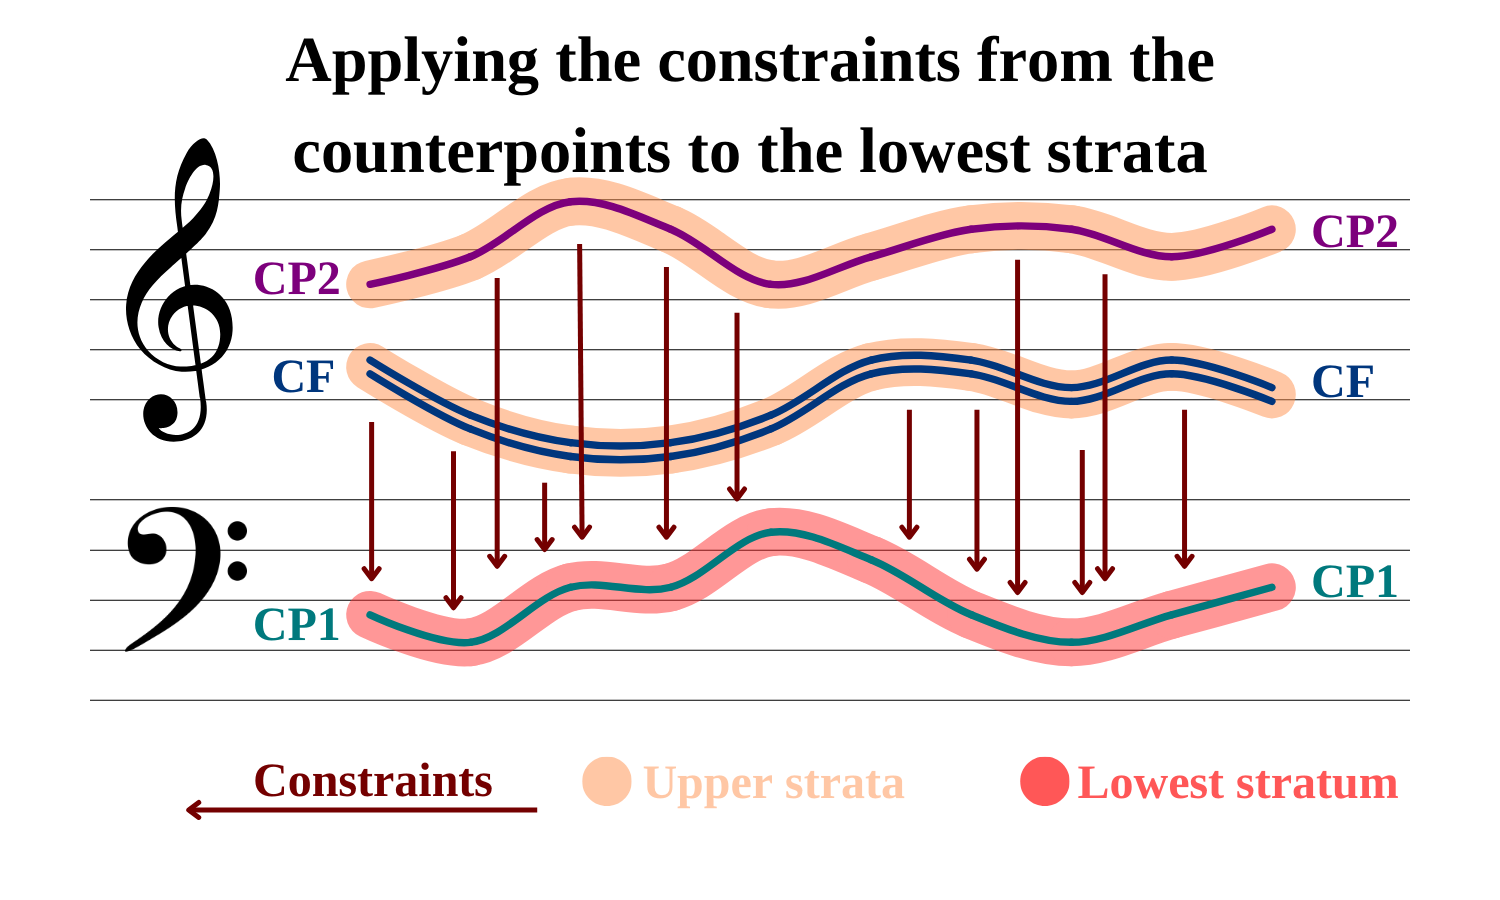
\includegraphics[width=\textwidth]{Images/p2l-3v.png}
      \captionof{figure}{Correct approach: applying the constraints between the parts to the lowest stratum.}
      \label{fig:p2l-3v}
\end{minipage}
\vspace{.5cm}

It is, of course, possible for the \cfs to be equal to the lowest stratum all along, in which case nothing changes from the perspective we had when composing for two voices. In this particular case, by applying the rules with respect to the \cf, we would find ourselves de facto applying the rules with respect to the lowest stratum (and we would be back to the situation described above, see figures \ref{fig:cp2cf-3v} and \ref{fig:p2l-3v}, only that there is now one more part). It is when the \cfs pitches are higher up than those of the counterpoints that considering the lowest stratum consideration becomes necessary.

\paragraph{TODO} complement the following paragraph to make it clearer
\paragraph{}
A very important detail, and perhaps the biggest change brought about by this paradigm shift, is since we do not compute all voices with respect to the \cfs, but with respect to the lowest stratum, it is important that the relationship between the \cfs and the lowest stratum also get taken into account. This means, when applying the constraints over the parts, we are considering the \cfs too (as it is a part, like the counterpoints), unless explicitely mentioned otherwise (for example in the variety cost). 

A second point to bear in mind, and not the least, is that all this does not mean that \textit{all} the rules are established between the parts and the lowest stratum. Certain rules will continue to apply between the different parts, regardless of whether they are high, low or intermediate.

\section{Changes induced in the variables} \label{section:changes induced}

Many changes have been induced as a result of the three part generalisation. In two part composition, it was obvious that the harmonic intervals array was describing the intervals between the \cfs and the only counterpoint, it was obvious that the motions were those of the only counterpoint, and so it goes for all the variables. When writing a three part composition, we are dealing with many possibilities when speaking about intervals or motions. Intervals between which voices? Motions of which counterpoint? To tackle this, each variable is now related to a voice.

This relationship between a variable and a voice is expressed as function. $X(v)$ represents the variable $X$ of the voice $v$. The arguments of the function can either be:
\begin{itemize}
    \item $\mathit{cf}$ - for linking the variable to the \cf.
    \item $cp_1$ - for linking the variable to the second \cp.
    \item $cp_2$ - for linking the variable to the third \cp.
    \item $a$ - for linking the variable to the lowest stratum.
    \item $b$ - for linking the variable to the intermediate stratum.
    \item $c$ - for linking the variable to the uppermost stratum.
  \end{itemize}

\noindent For example, $X(\mathit{cf})$ refers to the variable $X$ of the \cf.

\paragraph{}
When a variable is not explicitly linked to a voice, it is implied that the relation expressed for it is true for all \textit{parts}. In other words, if the variable $X$ is written without any precision, it means $X \equiv \forall v \in \{\mathit{cf}, cp_1, cp_2\}: X(v)$.

\paragraph{}
\noindent This change applies to all variables, namely:
\begin{itemize}
    \item \textbf{N}(v) - the notes (pitches) of voice v (this variable was written cp in T. Wafflard's thesis)
    \item \textbf{H}(v$_1$, v$_2$) - the harmonic intervals between voice v$_1$ and voice v$_2$. This variable is particular, as it needs to arguments to be meaningful.
    \item \textbf{M}(v) - the melodic intervals of voice v, 
    \item \textbf{P}(v) - the motions of voice v, 
    \item \textbf{IsCfB}(v) - the boolean array representing whether the cantus firmus is lower than a given voice,
    \item \textbf{IsCons}(v) - to the boolean array representing whether voice v is consonant or not.
\end{itemize}

\noindent It also applies to \textit{some} constants, namely:
\begin{itemize}
    \item \textbf{species}(p) - the species of part p,
    \item \textbf{n}(p) - the number of notes in part p,
    \item \textbf{lb}(p) - the lower bound of the range of part p,
    \item \textbf{ub}(p) - the upper bound of the range of part p,
    \item $\mathcal{R}$(p) - the range of part p,
    \item \textbf{borrow}(p) - the borrowing scale of part p,
    \item $\mathcal{N}$(p) - the extended domain of part p,
    \item $\mathcal{B}$(p) - the set of beats\footnote{To make it clearer: for the first species, the only beat in a measure is $\{0\}$, as there is only a note on the first beat. For the second species, the set of beats is $\{0, 2\}$. For the third species, it is: $\{0, 1, 2, 3\}$. For the fourth species: $\{0, 2\}$. And for the fifth species: $\{0, 1, 2, 3\}$.} in a measure according to the species of part p,
    \item b(p) - the number of beats\footnote{Thus, it is always equal to the size of the set $\mathcal{B}$(p).} in a measure according to the species of part p,
    \item d(p) - the duration of a note\footnote{For the first species, it is equal to $1$, as each note is a whole note. For the second species, it is $\dfrac{1}{2}$, and so on. It is always equal to $\dfrac{1}{b(p)}$.} according to the species of part p.
\end{itemize}
Please note that the constants cannot be linked to a stratum, and only to a part. Indeed, it would have no sense to speak about the species or about the extended domain of a stratum.

The costs are also affected by the change, except for $\mathcal{C}$ (the cost factors) and $\tau$ (the total cost). The latter two remain global and are not duplicated.


To make sure that those notations are clear, here are some examples: the notation $N(a)$ corresponds to the variable representing the notes (pitches) of the lowest stratum, whereas $N(\mathit{cf})$ are the notes of the \cf. The species of the second counterpoint is written $species(c)$. If only $N$ is written, then the equation in which $N$ is located holds true for any possible part (not necessary stratum). That is, the relationship $N < 60$ would mean: the pitches \textit{of all parts} must be lower than a middle C (whose representation is 60 is Open Music).

\subsubsection{Note regarding the fourth species}\label{nota-bene-4th-species} Let's recall that the fourth species behaves in a particular way compared to the other species. Its beats are "shifted": its upbeat should be considered as the downbeat, and its downbeat as the upbeat of the previous measure. This means that in the majority of cases, the equations for the fourth species would have to be rewritten, swapping the 0 and 2 indexes (H[2, j] becomes H[0, j] and H[0, j+1] becomes H[2, j]). To avoid duplicating each of the equations (a first equation if it is not of the fourth species and a second equation if it is of the fourth species) and also to avoid equations that are too complex and difficult to read, it was decided that the index swap would be implicit. Except, of course, when a rule concerns only the fourth species: in this case, the indexes are written as they are.

\subsection{Added constants}
Here are described some added constants, that are useful throughout the whole work.

\vspace{.5cm} \noindent \textbf{NumberOfParts} \hspace{.2cm} \texttt{*N-PARTS}

This integer describes as many parts there are in a given problem. At this stage, it can either be equal to two (two-part composition) or to three (three-part composition). It is mainly used in the loops of the program as an end condition (\texttt{(dotimes (i *N-PARTS))})

\vspace{.5cm} \noindent \textbf{Cons$_{h\_triad}$} \hspace{.2cm} \texttt{H\_TRIAD\_CONS}

Set representing all consonances that belong to the harmonic triad

\subsection{Added variables}
\vspace{.5cm} \noindent \textbf{A} \hspace{.cm} \texttt{is-lowest} \label{is-lowest}
% expliquer en EN que on peut pas lambda(cp1) ET lambda(cf)

A is an array of boolean variables with a size of $m$, where each variable indicates whether the corresponding part is the lowest stratum. In other words, $A(v)$ is true if v is the lowest stratum. The notation "A" was chosen as the uppercase of "a", which itself represents the lowest stratum. 
It is also worth to be noted that only one of the parts can be the lowest stratum at the time. This does not mean that two parts cannot equal the lowest stratum at the same time, it \textit{is} indeed possible that two parts blend in unison in the final chord, and that both pitches are the lowest sounding notes. It means that only one of those two is going to be considered to \textit{be} the lowest stratum (and the other one will be the intermediate stratum). This is needed in order for motions to work well. See \ref{subsubsection:one-part-per-stratum} for the details.

Here is the mathematical definition of the A array:
\begin{equation}
\begin{aligned}
\forall j \in [0, m-1)& \colon  \\
A(cf)[j] &= \,  
\begin{cases}
    \top & \text{if } N(cf)[0,j] = N(a)[0,j] \\
    \bot & \text{else }
\end{cases}\\
A(cp_1)[j] &= \,  
\begin{cases}
    \top & \text{if } (N(cp_1)[0,j] = N(a)[0,j]) \land \neg A(cf)[j] \\
    \bot & \text{else }
\end{cases}\\
A(cp_2)[j] &= \,  
\begin{cases}
    \top & \text{if } \neg A(cf) \land \neg A(cp_1)\\
    \bot & \text{else }
\end{cases}
\end{aligned}
\end{equation}

As can be seen in these equations, only the downbeat of each measure is taken into account when computing the A array. The reason for this is that it is the downbeat note that determines which chord will be \textit{the} chord of the measure, and the other beats are just fioritures. Another reason for this is also that it is only going to serve in contexts where the first note of the measure is relevant.

\paragraph{}
In practice, there is only an \texttt{is-not-bass} array in the code (which is then equal to $\neg A$), as it is almost always more useful to know if a part is \textit{not} the lowest stratum than knowing if it is the lowest one. 

\subsection{Modified constants} \label{subsection:modified_constants}
\noindent \textbf{species} \hspace{.2cm} \texttt{species} 

The species constant, which represents the species of a given part, can now take also take the value zero. The value zero is specific to the \cfs (which can be understood as a simplified first species counterpoint). This constant is more useful in the code than in the mathematical notations.
\begin{equation}
species(v) = 0 \iff v = cf
\end{equation}

\subsection{Redefined variables with respect to the definitions in T. Wafflard's thesis} \label{subsection:modified_variables}
Given that the majority of the rules now apply between parts and the lowest stratum, the meaning of the variables has been modified to adapt to this reality.
\paragraph{TODO} maybe mention also the variables that didn't change 

\paragraph{Nota bene}
Please take into consideration that all rules from T. Wafflard's thesis are compatible with the new definitions of the variables, as discussed in \ref{exploring-interaction-p-a}.

\vspace{.5cm} \noindent \textbf{N}(v) \hspace{.2cm} \texttt{notes} 

We changed the name of former \texttt{cp} array and renamed it to \texttt{N} (for notes), for the sake of clarity. As we have now three of those arrays (one for the first counterpoint, one for the second counterpoint, and even one for the \cf), it needed a less ambiguous name than the one it had before.
It still works exactly the same. It is an array of size $s_m$ representing the pitches of a given voice at a given beat in a measure.



\vspace{.5cm} \noindent \textbf{H}$_{(\text{abs})}$(v$_1$, v$_2$) \hspace{.2cm} \texttt{h-intervals}\hspace{.2cm} \texttt{h-intervals-abs}\hspace{.2cm} \texttt{h-intervals-to-cf}\hspace{.2cm}  ...

This variable keeps being an array of size $s_m$ and the way in which it works remains pretty much the same, i.e. it represents the harmonic interval between one voice and another. The previous definition of this array was that it represented the harmonic intervals between a given voice and the \cf. This definition has been extended to include intervals other than that between the counterpoint and the \cf. In order to do so, H accepts two arguments, and it represents the interval between those two arguments. Thus, $H(v1,v2)[i,j]$ represents the intervals between the $i$th beat of voice $v_1$ and the \textit{first} beat of voice $v_2$. $v_1$ may be a part and $v_2$ may be a stratum, as you can calculate harmonic intervals between a part and a stratum. When no $v_2$ is precised, it is equal to $a$, by default. In other words, $H(v_1)$ represents the intervals between the voice $v_1$ and the lowest stratum: $H(v_1) \equiv H(v_1,a)$. This default value for $v_2$ was chosen since it is the most frequently used, and for a good reason: most relevant harmonic intervals are those between the parts and the lowest stratum.

Here is the generalisation explained above, matching to the current definition of the harmonic intervals array:
\begin{equation}
\begin{aligned}
    &\forall v_1, v_2 \in \{cf, cp_1, cp_2, a, b, c\}, \quad \forall i \in \mathcal{B}(v_1), \quad \forall j \in [0, m):\\
    &H_{abs}(v_1,v_2)[i, j] = \left|N(v_1)[i, j] - N(v_2)[0,j]\right|\\
    &H(v_1-v_2)[i, j] = H_{abs}[i, j]\ \text{mod}\ 12\\
    &\text{where } H_{abs}[i, j] \in [0, 127], H[i, j] \in [0, 11]
\end{aligned}
\end{equation}

\vspace{.5cm}
\noindent \textbf{M}$_{\text{brut}}$(v) \hspace*{.2cm} \texttt{m-intervals-brut}

The variable M keeps representing the melodic intervals of a voice. It can either be evaluated on a part or on a stratum, each of those situations leading to different behaviours. M(p) (i.e. when related to a part) keeps representing the melodic intervals of the voice v and its way of working remains intact as in T. Wafflard's thesis. M(s) (i.e. when related to a stratum) has it own way of working, that is defined in the next paragraph. We are going to focus specifically on M(a), that is, the melodic intervals of the lowest stratum.

Since strata don't have melodic intervals \textit{per se} (they actually do have melodic intervals, but it doesn't really make sense to consider them), we need to redefine what we mean when speaking about the melodic intervals of a stratum. If it is not clear why strata have no inherent melodic intervals, remember that they are an abstract concept that is used only in mathematical relationships (and respective constraints). People who listen to the music hear the different parts (be they different tessitura, different instruments, ...) and the way these parts interact together in melodic movements and harmonic convergences, rendering a beautiful music, or not. Strata are an abstraction of the harmonic interactions between the parts, and because of this, they are a consequence of the parts: they exist because the parts exist, and not the other way round! And since they are defined according to harmonic principles (as was suggested before, they are successions of vertical alignments), speaking about the proper \textit{melodic} intervals of a stratum makes no sense. One could then conclude that melodic intervals do not apply to strata, and go ahead. Nevertheless, Fux \textit{does} speak about computing the motions between a part and the lowest stratum. And to be able to compute motions, one needs to compare two different melodic intervals. So we need to have a definition for the melodic intervals of a stratum. 

In order to do so, one must recall that the lowest stratum is just the assemblage of all the lowest sounding notes in the composition. It is thus very logical to consider the melodic intervals of the lowest stratum as the melodic intervals that lead to all those lowest sounding notes. If the lowest stratum is constituted of the notes [C$_{cp_1}$, E$_{cf}$, G$_{cp_2}$], with C$_{cp_1}$ indicating that the C belongs to the first \cp, and  and that in the \cfs the interval that lead to the E was a +0 (i.e. staying on the same note) and in the second \cps the interval that lead to the G was a -4 (getting down of two tones), the corresponding melodic intervals array of the lowest stratum would be [+0, -2]. This example has been written again in a more visual way in equation \ref{eq:defining-m-intervals-bass} to make it easier to understand:



\begin{equation}
    \begin{aligned}        
    N(cf) &= [64,\quad  \textcolor{darkred}{\textbf{64}},\quad  71] \quad 
    &M_{brut}(cf) &= [\textcolor{darkred}{\textbf{+0}}, \quad +7]\\
    N(cp_1) &= [\textcolor{darkred}{\textbf{60}},\quad  67,\quad  74] \quad 
    &M_{brut}(cp_2) &= [+7, \quad +7]\\
    N(cp_2) &= [72,\quad  71,\quad  \textcolor{darkred}{\textbf{67}}] \quad 
    &M_{brut}(cp_2) &= [-1, \quad \textcolor{darkred}{\textbf{-4}}]\\
    \\
    N(a) &= [\textcolor{darkred}{\textbf{60}},\quad  \textcolor{darkred}{\textbf{64}},\quad  \textcolor{darkred}{\textbf{67}}] \quad 
    &M_{brut}(a) &= [\textcolor{darkred}{\textbf{+0}}, \quad \textcolor{darkred}{\textbf{-4}}]\\
\end{aligned}
\label{eq:defining-m-intervals-bass}
\end{equation}


The formal definition of the melodic intervals of the lowest stratum is hence as follows: the melodic interval in measure $j$ of the lowest stratum is equal to the last melodic interval in measure $j$ of the part that is the lowest stratum in measure $j+1$. Remember that this complex definition is needed in order for the computation of the motions to work fine, and that the motions of the lowest stratum are an abstract notion that serves only in formulas and constraints and \textit{does not intend to represent any concrete motion really happening in the composition, nor does it correspond to the melodic intervals between the pitches of the lowest stratum}.

\begin{equation}
    \begin{aligned}
        &\forall j \in [0, m-2):\\
        &M_{brut}(a)[j] = \,  
        \begin{cases}
            M_{brut}(cf)[0][j] & \text{if } A(cf)[j+1]\\
            M_{brut}(cp_1)[\text{max}(\mathcal{B}(cp_1))][j] & \text{if } A(cp_1)[j+1]\\
            M_{brut}(cp_2)[\text{max}(\mathcal{B}(cp_1))][j] & \text{if } A(cp_2)[j+1]\\
        \end{cases}
    \end{aligned}
\end{equation}

\noindent It might be helpful to have a look at figures \ref{fig:stratum-m-intervals-1} and \ref{fig:stratum-m-intervals-2} to understand better how the melodic intervals arrays for the lowest stratum.

\vspace{.5cm}
\begin{minipage}{0.46\textwidth}
    \centering
    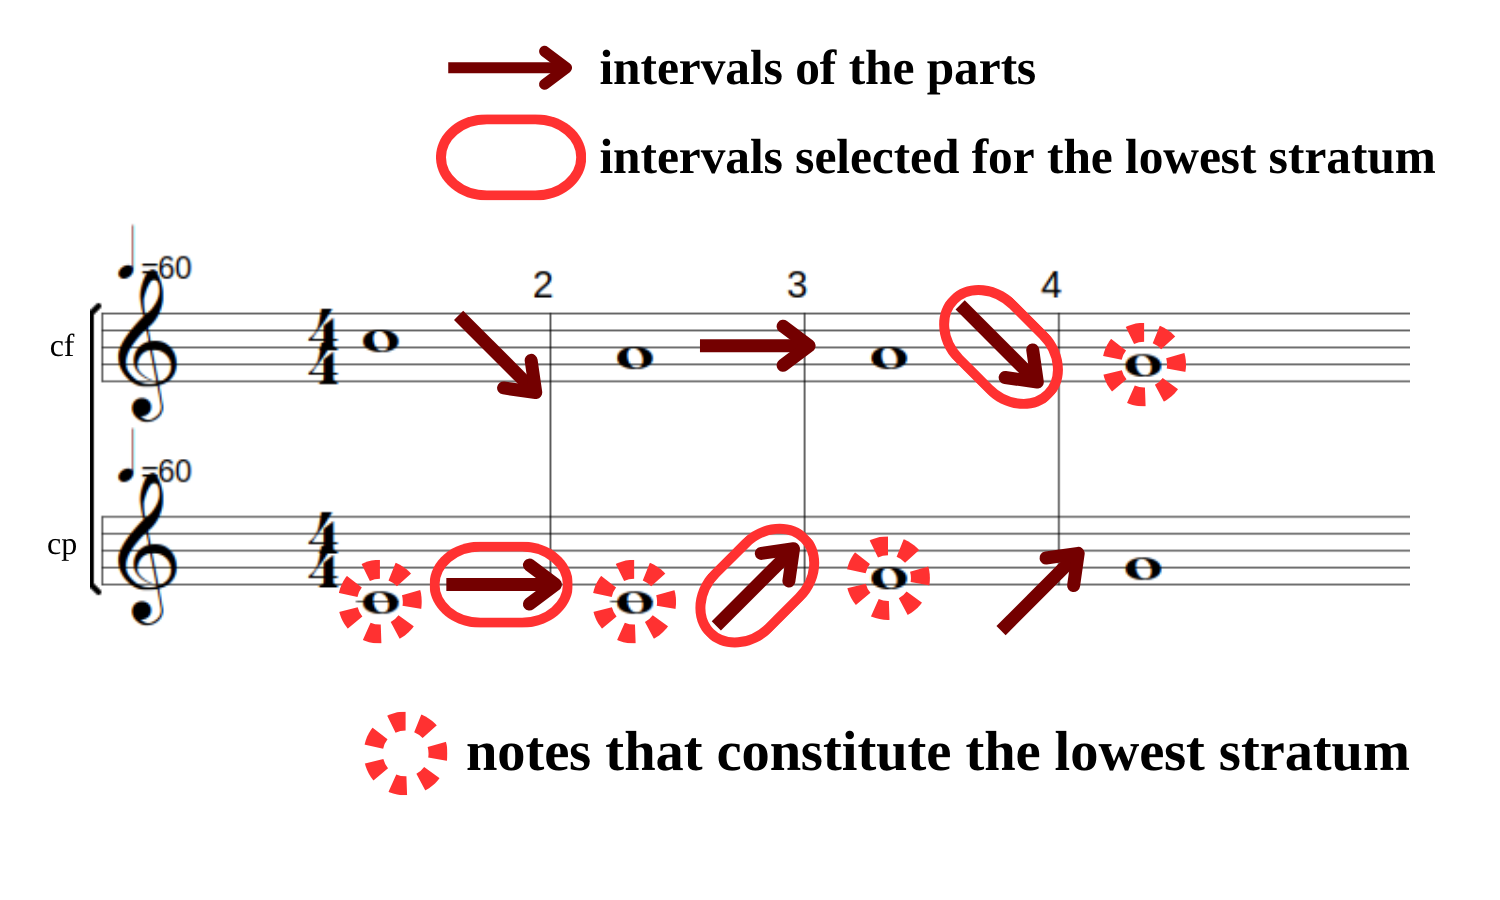
\includegraphics[width=\textwidth]{Images/stratum-m-intervals.png}
    \captionof{figure}{Understanding the melodic intervals of the lowest stratum with a first species counterpoint}
    \label{fig:stratum-m-intervals-1}
    \end{minipage}
    \hfill
    \begin{minipage}{0.46\textwidth}
      \centering
      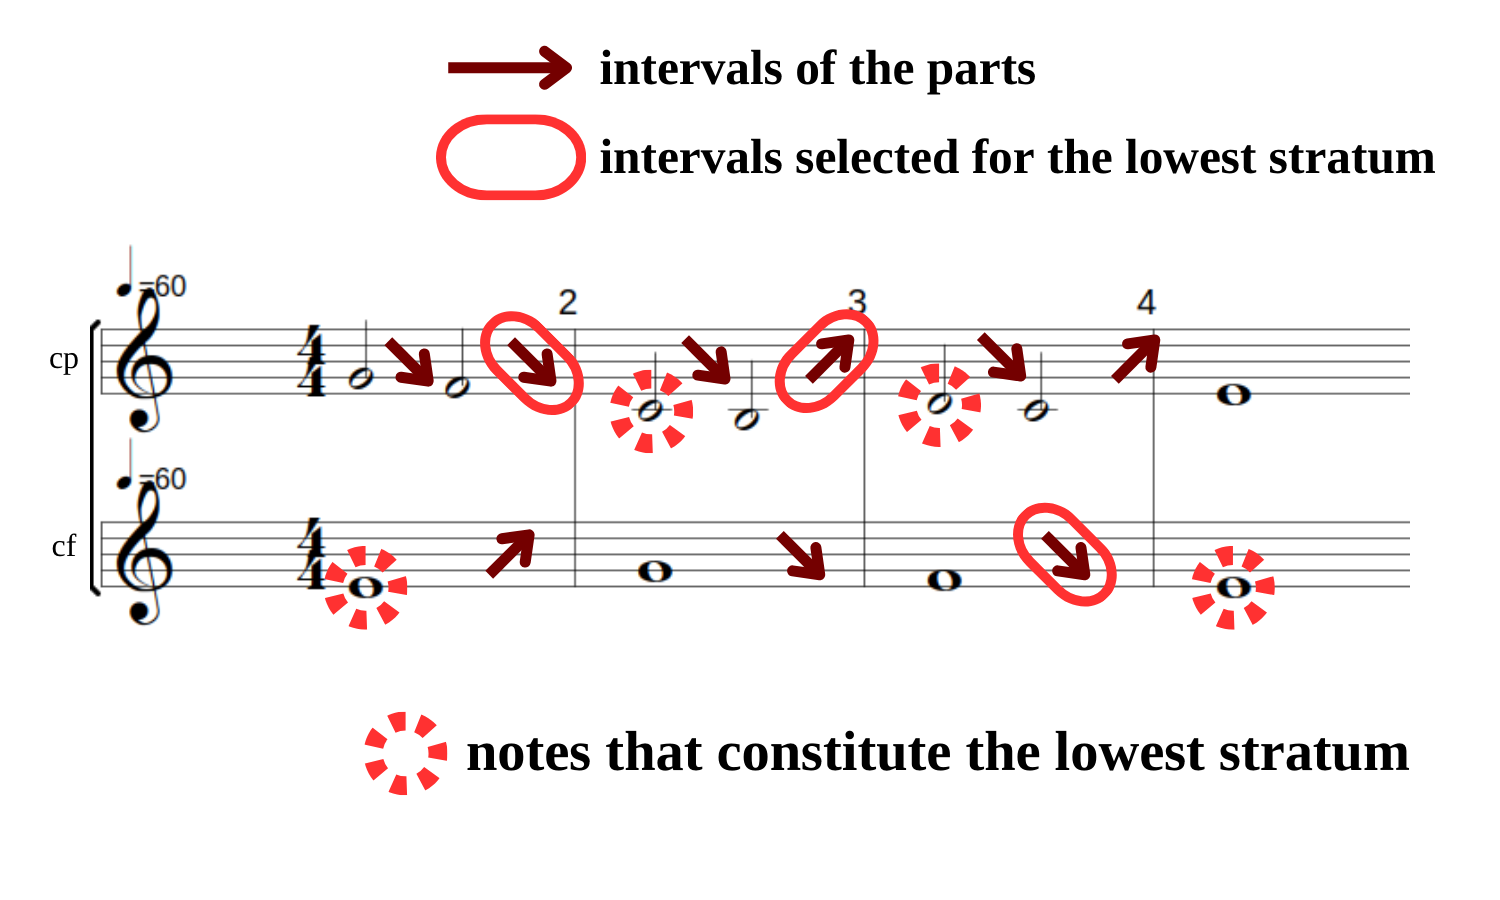
\includegraphics[width=\textwidth]{Images/stratum-m-intervals2.png}
      \captionof{figure}{Understanding the melodic intervals of the lowest stratum with a second species counterpoint}
      \label{fig:stratum-m-intervals-2}
\end{minipage}


\vspace{.5cm}
\noindent \textbf{P}(p) \hspace*{.2cm} \texttt{motions}

The motions array was redefined to compute the motions of a voice v with respect to the lowest stratum, instead of computing them with respect to the \cf, since Fux considers that the motions should be considered between each voice and the lowest voice. Dealing with the melodic intervals of the lowest stratum is not a problem anymore, since we defined what it exactly means in the section about melodic intervals.
However, a problem arises when computing the motions of the part that is also the lowest stratum in some measures. When this happens, we end up calculating motions between a part and itself. Any part is inevitably moving in direct motion with itself, and this situation leads to only direct motions being calculated. This becomes problematic when considering costs (it is bad to have direct motions, but it obviously should not be bad to be the lowest stratum), and when considering some constraints. To tackle this problem, the motions of a part are now equal to -1 when the part is also the lowest stratum (which is denoted A(p), see section \ref{is-lowest}). 
\begin{equation}
\begin{aligned}
&\forall p \in \{cf, cp_1, cp_2\}, \quad \forall x \in \{1, 2\}, \quad \forall i \in B, \quad \forall j \in [0, m - 1),\quad x := b - i\\
    &motion(p)[i,j] = \,  
    \begin{cases}
        0 & \land (M_{brut}^{x}(p)[i, j] > 0 > M(a)_{brut}[j]) \\ & \quad \quad \quad \quad \quad \quad \quad \quad \quad  \vee (M_{brut}^{x}(p)[i, j] < 0 < M(a)_{brut}[j]) \\
        1 & M_{brut}^{x}(p)[i, j] = 0  \oplus M(a)_{brut}[j]=0 \\
        2 & (M_{brut}^{x}(p)[i, j] > 0 \land M(a)_{brut}[j] > 0) \\ & \quad \quad \quad \quad \quad \quad \quad \quad \quad   \vee  (M_{brut}^{x}(p)[i, j] < 0 \land M(a)_{brut}[j] <0)
    \end{cases} 
    \\
    &P(p)[i,j] = \,  
    \begin{cases}
        -1 & \text{if } A(p)[j] \\
        motion(p)[i,j] & \text{if } \neg A(p)[j]
    \end{cases}
\end{aligned}
\end{equation}
